\documentclass[12pt,a4paper]{article}

% ---------------------------------------------------------------
% Packages
% ---------------------------------------------------------------
\usepackage[margin=1in]{geometry}
\usepackage{amsmath, amsthm, amssymb}
\usepackage{algorithm}
\usepackage{algpseudocode}
\usepackage{booktabs}
\usepackage{array}
\usepackage{tabularx}
\usepackage{hyperref}
\usepackage{parskip}
\usepackage{enumitem}
\usepackage{setspace}
\usepackage{fancyhdr}
\usepackage{titlesec}
\usepackage{caption}
\usepackage{graphicx}

\onehalfspacing

% ---------------------------------------------------------------
% Theorem environments
% ---------------------------------------------------------------
\newtheorem{theorem}{Theorem}[section]
\newtheorem{lemma}[theorem]{Lemma}
\theoremstyle{definition}
\newtheorem{definition}{Definition}[section]

% ---------------------------------------------------------------
% Header / footer
% ---------------------------------------------------------------
\pagestyle{fancy}
\fancyhf{}
\rhead{CS 301 -- Project Report}
\lhead{Subset Sum}
\cfoot{\thepage}

% ---------------------------------------------------------------
% Algorithmic settings
% ---------------------------------------------------------------
\algnewcommand{\LineComment}[1]{\State \texttt{//} #1}
\renewcommand{\algorithmicrequire}{\textbf{Input:}}
\renewcommand{\algorithmicensure}{\textbf{Output:}}

% ---------------------------------------------------------------
\begin{document}

% ---------------------------------------------------------------
% Title page
% ---------------------------------------------------------------
\begin{titlepage}
  \centering
  \vspace*{2cm}
  {\Large CS 301}\\[0.4cm]
  {\large 2025--2026 Spring}\\[1.5cm]
  {\Huge \textbf{Project Report}}\\[1.5cm]
  {\large Group 15}\\[0.8cm]
  {\normalsize
    \textbf{Group Members:}\\[0.3cm]
    Musab Ahmed Khan \quad 33017\\
    Imran Hasanzade \quad 33537\\
    Umar Hanif Abdul Aziz \quad 32758
  }
  \vfill
\end{titlepage}

% ---------------------------------------------------------------
% Table of contents
% ---------------------------------------------------------------
\tableofcontents
\newpage

% ===============================================================
\section{Problem Description}
% ===============================================================

\begin{table}[h!]
  \centering
  \renewcommand{\arraystretch}{1.4}
  \begin{tabular}{>{\bfseries}p{2.5cm} p{10cm}}
    \toprule
    Name     & Subset Sum \\
    \midrule
    Input    & A finite set $S = \{s_1, s_2, \ldots, s_n\}$ of integers
               and a target integer $k$ \\
    Question & Does there exist a subset $T \subseteq S$ such that
               $\displaystyle\sum_{s \in T} s = k$? \\
    \bottomrule
  \end{tabular}
  \caption{Description of the Subset Sum Problem}
\end{table}

% ---------------------------------------------------------------
\subsection{Overview}
% ---------------------------------------------------------------

The Subset Sum problem is one of the most studied problems in computer science.
Given a set of integers and a target value, the question is whether some subset
of those integers adds up to exactly that target. In the optimization version, the
goal is to find the subset whose sum is as large as possible without exceeding the target.

The problem is easy to state, but hard to solve in general. No known algorithm
handles all instances efficiently. It has been proven to be NP-complete, meaning
it belongs to a class of problems for which no polynomial-time algorithm is
expected to exist unless $\mathrm{P} = \mathrm{NP}$.

% ---------------------------------------------------------------
\subsection{Decision Problem}
% ---------------------------------------------------------------

The decision version asks a yes-or-no question:

\begin{quote}
  \textit{Given a finite set $S = \{s_1, s_2, \ldots, s_n\}$ of integers and
  a target integer $k$, does there exist a subset $T \subseteq S$ such that
  $\sum_{s \in T} s = k$?}
\end{quote}

Formally:
\[
  \mathrm{SUBSET\text{-}SUM}
    = \bigl\{\langle S,\, k \rangle
       \mid \exists\, T \subseteq S \text{ such that } \textstyle\sum_{s \in T} s = k
      \bigr\}
\]

For example, given $S = \{3, 1, 4, 2, 6\}$ and $k = 7$, the answer is YES
because $\{1, 6\}$ sums to 7. If $k = 17$, the answer is NO because the
total sum of all elements is only 16, so no subset can reach 17.

% ---------------------------------------------------------------
\subsection{Optimization Problem}
% ---------------------------------------------------------------

The optimization version does not ask whether a solution exists. It asks for
the best feasible one:

\begin{quote}
  \textit{Given a finite set $S = \{s_1, \ldots, s_n\}$ of non-negative integers
  and a target $k$, find a subset $T \subseteq S$ that maximizes
  $\sum_{s \in T} s$ subject to $\sum_{s \in T} s \leq k$.}
\end{quote}

If a subset summing to exactly $k$ exists, that is trivially optimal. Otherwise
the goal is to get as close to $k$ as possible from below.

Note: in the experimental sections of this report, only the optimization version
is tested. For the decision version, the test is simply whether the algorithm
returns a subset summing to exactly $k$.

% ---------------------------------------------------------------
\subsection{Example Illustration}
% ---------------------------------------------------------------

\textbf{Example 1 (Decision: YES).}
Let $S = \{4, 11, 16, 21, 27\}$ and $k = 25$. The subset $\{4, 21\}$ sums to
25. The decision answer is YES.

\textbf{Example 2 (Decision: NO; Optimization returns near-optimal).}
Let $S = \{5, 7, 12\}$ and $k = 10$. No subset sums to exactly 10.
The feasible subsets (those with sum $\leq 10$) and their sums are:

\begin{center}
  \begin{tabular}{ll}
    \toprule
    Subset & Sum \\
    \midrule
    $\{\}$   & 0 \\
    $\{5\}$  & 5 \\
    $\{7\}$  & 7 \\
    \bottomrule
  \end{tabular}
\end{center}

The decision answer is NO. The optimization answer is $\{7\}$ with sum 7.

\textbf{Example 3 (k equals sum of all elements).}
Let $S = \{4, 6, 10\}$ and $k = 20$. The full set $\{4, 6, 10\}$ sums to 20.
Both the decision and optimization answers return the full set.

\textbf{Example 4 (All elements exceed k).}
Let $S = \{10, 20, 30\}$ and $k = 5$. No non-empty subset is feasible.
The optimization answer is the empty set with sum 0.

% ---------------------------------------------------------------
\subsection{Real-World Applications}
% ---------------------------------------------------------------

\textbf{Resource allocation and budgeting.}
A direct application is deciding whether a collection of tasks or items with
associated costs can exactly fill a given budget. For instance, selecting jobs
from a list so that their total processing time exactly matches an available
time slot is an instance of Subset Sum.

\textbf{Cryptography.}
The Merkle-Hellman knapsack cryptosystem, one of the earliest public-key
schemes, is built directly on the hardness of Subset Sum~\cite{garey}. Encryption
maps a message to a subset sum of a public key; decryption uses a hidden
trapdoor that converts the hard instance into an easy one.

\textbf{Load balancing.}
Distributing a set of jobs across processors so that each processor carries
the same total load is equivalent to a partition problem, which is a special
case of Subset Sum.

\textbf{Finance and auditing.}
Identifying whether a set of transactions can exactly account for a given
total is a direct use of the decision version, and appears in reconciliation
and audit workflows.

% ---------------------------------------------------------------
\subsection{Hardness of the Problem}
% ---------------------------------------------------------------

\begin{theorem}
  The decision version of the Subset Sum problem is NP-complete.
\end{theorem}

The proof has two parts.

\subsubsection{Proving NP}

A problem is in NP if a proposed solution can be verified in polynomial time.
For Subset Sum, the certificate is the subset $T$ itself. Given $T$, we verify
it by computing $\sum_{s \in T} s$ and checking whether it equals $k$. This
takes $O(n)$ time. Therefore, Subset Sum $\in$ NP~\cite{sipser} (Theorem~7.25,
p.~297).

\subsubsection{Proving NP-Hard}

Karp~\cite{karp} proved that Subset Sum is NP-hard by showing a polynomial-time
reduction from the 3-SAT problem. Since 3-SAT is NP-complete and every
NP problem reduces to it in polynomial time, a polynomial-time reduction from
3-SAT to Subset Sum implies that Subset Sum is at least as hard as any
problem in NP. The complete reduction is given in~\cite{sipser} (Section~7.5,
p.~319) and in the original paper~\cite{karp}. We cite these rather than
reproduce the proof here.

\subsubsection{Proving NP-Complete}

Since Subset Sum is both in NP and NP-hard, it is NP-complete. This means
that unless $\mathrm{P} = \mathrm{NP}$, no polynomial-time algorithm correctly
solves all instances. The brute-force algorithm in Section~2.1 therefore has
exponential worst-case time, and the heuristic in Section~2.2 trades optimality
for efficiency.


% ===============================================================
\section{Algorithm Description}
% ===============================================================

\subsection{Brute Force Algorithm}

\subsubsection{Overview}

The brute force algorithm solves the Subset Sum problem by checking every
possible subset of $S$. For a set of $n$ elements there are $2^n$ subsets in
total, including the empty set. The algorithm evaluates each one and either
checks for an exact match (decision version) or tracks the best feasible sum
found so far (optimization version).

The implementation uses bitmask enumeration. Each integer in the range
$[0,\, 2^n - 1]$ is treated as a binary string of length $n$, where bit $i$
indicates whether element $S[i]$ is included. This lets all $2^n$ subsets be
generated with a single loop.

This is pure exhaustive search. It does not use divide-and-conquer or dynamic
programming. It is guaranteed to find the correct answer because it examines
every candidate without exception. The trade-off is that its runtime grows
exponentially with $n$, making it impractical beyond roughly $n = 25$. Its
main role in this project is to provide a correct reference solution for the
quality-testing experiments in Section~7.

\subsubsection{Pseudocode}

Algorithm~\ref{alg:bf-opt} gives the optimization version. The decision version
follows the same structure but returns as soon as a subset summing to exactly
$k$ is found.

\begin{algorithm}[H]
\caption{Brute Force Optimization}
\label{alg:bf-opt}
\begin{algorithmic}[1]
\Require Set $S = [s_0, \ldots, s_{n-1}]$, target $k$
\Ensure Subset of $S$ with maximum sum $\leq k$
\State $\textit{best\_sum} \gets 0$
\State $\textit{best\_subset} \gets [\,]$
\For{$\textit{mask} \gets 0$ \textbf{to} $2^n - 1$}
    \State $\textit{current\_sum} \gets 0$
    \State $\textit{current\_subset} \gets [\,]$
    \For{$i \gets 0$ \textbf{to} $n - 1$}
        \If{bit $i$ of \textit{mask} is set}
            \State $\textit{current\_sum} \gets \textit{current\_sum} + S[i]$
            \State $\textit{current\_subset}.\mathrm{append}(S[i])$
        \EndIf
    \EndFor
    \If{$\textit{current\_sum} \leq k$ \textbf{and} $\textit{current\_sum} > \textit{best\_sum}$}
        \State $\textit{best\_sum} \gets \textit{current\_sum}$
        \State $\textit{best\_subset} \gets \textit{current\_subset}$
    \EndIf
    \If{$\textit{best\_sum} = k$}
        \State \textbf{break} \Comment{exact match found, no improvement possible}
    \EndIf
\EndFor
\State \Return $\textit{best\_subset},\; \textit{best\_sum}$
\end{algorithmic}
\end{algorithm}

\begin{algorithm}[H]
\caption{Brute Force Decision}
\label{alg:bf-dec}
\begin{algorithmic}[1]
\Require Set $S = [s_0, \ldots, s_{n-1}]$, target $k$
\Ensure (\textsc{Found}, subset) if a subset sums to $k$, else (\textsc{Not Found}, $[\,]$)
\For{$\textit{mask} \gets 0$ \textbf{to} $2^n - 1$}
    \State $\textit{current\_sum} \gets 0$; \quad $\textit{current\_subset} \gets [\,]$
    \For{$i \gets 0$ \textbf{to} $n - 1$}
        \If{bit $i$ of \textit{mask} is set}
            \State $\textit{current\_sum} \gets \textit{current\_sum} + S[i]$
            \State $\textit{current\_subset}.\mathrm{append}(S[i])$
        \EndIf
    \EndFor
    \If{$\textit{current\_sum} = k$}
        \State \Return (\textsc{Found}, $\textit{current\_subset}$)
    \EndIf
\EndFor
\State \Return (\textsc{Not Found}, $[\,]$)
\end{algorithmic}
\end{algorithm}

The early exit at line~16 of Algorithm~\ref{alg:bf-opt} is a minor
optimization: once an exact match is found, the result is already optimal and
no further subsets need to be checked. Without it, the algorithm still produces
the correct answer but always runs for all $2^n$ iterations.

\medskip
\noindent\textit{Design technique.} Pure exhaustive search. No divide-and-conquer
or dynamic programming structure is used.

% ---------------------------------------------------------------
\subsection{Heuristic Algorithm}
% ---------------------------------------------------------------
\subsubsection{Overview}

The algorithm chosen for this problem is a fully polynomial-time approximation scheme
(FPTAS)~\cite{clrs} (Section~35.5). An approximation scheme is a type of approximation algorithm
that has the ability to achieve better and better approximation at the cost of more
computation time.

More specifically, an approximation scheme algorithm takes an additional input value
$\varepsilon$ such that, for any fixed $\varepsilon$, the scheme becomes a
$(1+\varepsilon)$-approximation algorithm. This means that the ratio of the calculated
approximation cost compared to the optimal cost is bounded by $1+\varepsilon$, but at
the expense of having the running time affected by this $\varepsilon$ value. For example,
it may have a running time of $O(n^2/\varepsilon)$, which causes the running time to
increase rapidly as we decrease $\varepsilon$ to get a better approximation.

We say that an algorithm is a fully polynomial-time approximation scheme if it is an
approximation scheme and it has a running time that is polynomial with respect to both
$1/\varepsilon$ and the input size $n$. For example, $O((1/\varepsilon)^2 n^3)$ is
fully polynomial. As can be seen, this running time increases based on the input size
and $1/\varepsilon$, but it increases in polynomial order and does not become exponential.

So our procedure:
\begin{itemize}
    \item takes as input a set $S$ consisting of $n$ integers,
    $S = \{x_1, x_2, \ldots, x_n\}$, a target integer $t$, and an approximation
    parameter $\varepsilon$, where $0 < \varepsilon < 1$;
    
    \item returns a value $z$ whose value is within a $1+\varepsilon$ factor of the
    optimal solution.
\end{itemize}

\noindent\textit{Note on notation.} This section follows the variable names used
in the original source~\cite{clrs}, where the target is denoted $t$. Elsewhere
in this report the target is called $k$; the two are interchangeable.

We use an iterative procedure that, in iteration $i$, computes the sums of all subsets
of $\{x_1, x_2, \ldots, x_i\}$ using as a starting point the sums of all subsets of
$\{x_1, x_2, \ldots, x_{i-1}\}$. A detailed explanation is given under the pseudocode,
as it is needed to understand the algorithm.

\subsubsection{Pseudocode}

\begin{algorithm}[H]
\caption{\textsc{Trim}$(L, \delta)$}
\begin{algorithmic}[1]
\State let $m$ be the length of $L$
\State $L' = \langle y_1 \rangle$
\State $last = y_1$
\For{$i = 2$ \textbf{to} $m$}
    \If{$y_i > last \cdot (1+\delta)$} \Comment{$y_i \geq last$ because $L$ is sorted}
        \State append $y_i$ onto the end of $L'$
        \State $last = y_i$
    \EndIf
\EndFor
\State \Return $L'$
\end{algorithmic}
\end{algorithm}

\begin{algorithm}[H]
\caption{\textsc{Approx-Subset-Sum}$(S,t,\varepsilon)$}
\begin{algorithmic}[1]
\State $n = |S|$
\State $L_0 = \langle 0 \rangle$
\For{$i = 1$ \textbf{to} $n$}
    \State $L_i = \textsc{Merge-Lists}(L_{i-1}, L_{i-1} + x_i)$
    \State $L_i = \textsc{Trim}(L_i, \varepsilon/2n)$
    \State remove from $L_i$ every element that is greater than $t$
\EndFor
\State let $z^*$ be the largest value in $L_n$
\State \Return $z^*$
\end{algorithmic}
\end{algorithm}

% ===============================================================
\section{Algorithm Analysis}
% ===============================================================

\subsection{Brute Force Algorithm}

\subsubsection{Correctness Analysis}

\begin{theorem}
  Algorithm~\ref{alg:bf-opt} correctly solves the Subset Sum optimization
  problem. That is, it returns a subset $T^* \subseteq S$ such that
  $\sum_{s \in T^*} s \leq k$ and this sum is maximum over all subsets of $S$
  with sum at most $k$.
\end{theorem}

\begin{proof}
The integers $0, 1, \ldots, 2^n - 1$ are in one-to-one correspondence with all
subsets of $S$: for any mask $m$, the set of indices $\{i : \text{bit } i
\text{ of } m \text{ is set}\}$ uniquely identifies a subset, and every subset
of $S$ corresponds to exactly one mask. Therefore the outer loop visits every
subset of $S$ exactly once.

For each visited subset, lines~12--14 update \textit{best\_sum} when the current
subset is feasible (sum $\leq k$) and strictly better than the previous best.
Since every subset is visited, the optimal feasible subset is visited at some
iteration. At that iteration, the condition on line~12 holds (the optimal sum
is $\leq k$ by definition and is at least as large as any prior feasible sum),
so \textit{best\_subset} is updated. By the end of the loop,
\textit{best\_subset} holds the optimal subset.

The early exit on lines~16--17 does not affect correctness: once
$\textit{best\_sum} = k$, no feasible subset can have a larger sum, so stopping
early yields the same result.
\end{proof}

\subsubsection{Time Complexity Analysis}

The outer loop runs for all integers from $0$ to $2^n - 1$, giving $2^n$
iterations. For each iteration, the inner loop on lines~6--11 runs $n$ times
(one bit check per element), and each step takes $O(1)$ time. The total
operation count is:
\[
  T(n) = 2^n \cdot n
\]
This is both an upper and a lower bound in the worst case (when no exact
solution exists and no early exit is triggered). Therefore the worst-case
time complexity is:
\[
  \boxed{T(n) = \Theta(n \cdot 2^n)}
\]
This is exponential in $n$. For $n = 20$ this is approximately $20 \times 10^6$
operations; for $n = 30$ it is around $30 \times 10^9$, which takes seconds
on typical hardware.

\subsubsection{Space Complexity Analysis}

The algorithm uses the following memory beyond the input array $S$:

\begin{itemize}[noitemsep]
  \item \textit{current\_subset} and \textit{best\_subset}: each stores at
        most $n$ elements, so $O(n)$ each.
  \item Scalar variables (\textit{mask}, $i$, \textit{current\_sum},
        \textit{best\_sum}): $O(1)$.
  \item No recursion is used, so there is no call-stack overhead beyond $O(1)$.
\end{itemize}

Total auxiliary space (not counting the input):
\[
  \boxed{O(n)}
\]

\subsection{Heuristic Algorithm}

\subsubsection{Correctness Analysis}

\begin{theorem}
  The \textsc{Approx-Subset-Sum} algorithm always returns a feasible result,
  and the returned value $z^*$ satisfies
  \[
    \frac{\mathrm{OPT}}{1+\varepsilon} \;\leq\; z^* \;\leq\; \mathrm{OPT},
  \]
  where $\mathrm{OPT}$ is the maximum subset sum not exceeding $k$.
\end{theorem}

The proof has two parts.

\paragraph{Feasibility.}
After each element $x_i$ is processed, every candidate whose sum exceeds $k$ is
explicitly removed from the list (line~6 of \textsc{Approx-Subset-Sum}). Since the
initial list contains only the value $0$ (the empty subset), and every candidate that
survives a step has sum at most $k$, all candidates in the final list $L_n$ are
feasible. The returned value $z^* = \max L_n$ is therefore at most $k$.

\paragraph{Approximation ratio.}
The key observation is that the \textsc{Trim} step may remove a candidate $y$ from the
list only when a representative $z$ with $z \leq y \leq z(1+\delta)$ is already
present. No candidate is dropped unless a nearby one remains to take its place.

Let $\delta = \varepsilon / (2n)$. By an inductive argument over the $n$ iterations,
one can show that after step $i$ the list $L_i$ contains a value $\hat{y}_i$ such that
\[
  \mathrm{OPT}_i \;\leq\; \hat{y}_i \cdot (1+\delta)^i,
\]
where $\mathrm{OPT}_i$ is the best achievable sum using the first $i$ elements.
At $i = n$ this gives $\mathrm{OPT} \leq z^* \cdot (1+\delta)^n$.

Bounding the accumulated error factor using $(1 + x)^n \leq e^{nx}$:
\[
  (1+\delta)^n
    = \!\left(1 + \frac{\varepsilon}{2n}\right)^{\!n}
    \leq e^{\,\varepsilon/2}.
\]
For $0 < \varepsilon \leq 1$, the inequality $e^x \leq 1/(1-x)$ and $x \leq 1/2$ give
$e^{\varepsilon/2} \leq 1 + \varepsilon$. Therefore:
\[
  \mathrm{OPT} \;\leq\; z^* \cdot (1+\varepsilon)
  \quad\Longrightarrow\quad
  z^* \;\geq\; \frac{\mathrm{OPT}}{1+\varepsilon}.
\]
The complete formal proof, including the inductive step, is given in~\cite{clrs}
(Theorem~35.7, Section~35.5).

Note: for the Subset Sum optimization problem, correctness in the context of a
heuristic means producing a valid feasible result, not necessarily the optimal one.
The approximation ratio above bounds how far from optimal the result can be.

\subsubsection{Time Complexity Analysis}

The bound on the list size drives the analysis. After \textsc{Trim} with
$\delta = \varepsilon/(2n)$, consecutive elements in the list differ by a factor of
more than $(1+\delta)$. If the smallest nonzero element is at least $1$ and the
largest is at most $t$ (the target), the number of elements in the list is at most:
\[
  \left\lfloor \log_{1+\delta}(t) \right\rfloor + 2
  \;=\; \left\lfloor \frac{\ln t}{\ln(1+\delta)} \right\rfloor + 2
  \;\leq\; \frac{\ln t}{\delta} + 2
  \;=\; \frac{2n\ln t}{\varepsilon} + 2
  \;=\; O\!\left(\frac{n \log t}{\varepsilon}\right).
\]
Call this bound $m$. Each of the $n$ outer iterations does the following work:
\begin{itemize}[noitemsep]
  \item Forming the shifted list ($L_{i-1} + x_i$): $O(m)$.
  \item Merging the two lists and sorting: $O(m \log m)$.
  \item Trimming: $O(m)$.
  \item Filtering elements above $t$: $O(m)$.
\end{itemize}
The dominant step per iteration is $O(m \log m)$. Over all $n$ iterations:
\[
  T(n,\varepsilon,t) \;=\; O\!\left(n \cdot m \log m\right)
  \;=\; O\!\left(\frac{n^2 \log t}{\varepsilon}
               \cdot \log\!\left(\frac{n \log t}{\varepsilon}\right)\right).
\]
Since $\log(n \log t / \varepsilon) = O(\log n + \log\log t + \log(1/\varepsilon))$,
this simplifies to:
\[
  \boxed{T(n,\varepsilon,t) \;=\; O\!\left(\frac{n^2 \log t \cdot \log(n/\varepsilon)}{\varepsilon}\right)}
\]
This is polynomial in $n$, $\log t$, and $1/\varepsilon$, which is exactly the condition
for an FPTAS. Note that a tight $\Theta$ bound is harder to establish here because the
list size depends on the actual values in each instance, so we state the $O$ bound.

\subsubsection{Space Complexity Analysis}

The candidate list at any step holds at most $m = O(n \log t / \varepsilon)$ pairs.
Our implementation stores each candidate as a pair \texttt{(sum, subset)}, where the
subset can contain up to $n$ elements. The space needed for the candidate list is
therefore:
\[
  O(m \cdot n) \;=\; O\!\left(\frac{n^2 \log t}{\varepsilon}\right).
\]
The algorithm also uses $O(n)$ space for the input $S$ and a constant number of
scalar variables. The dominant term is the candidate list, giving total auxiliary space:
\[
  \boxed{O\!\left(\frac{n^2 \log t}{\varepsilon}\right)}
\]
For the instances tested in Section~5.2 ($n \leq 130$, $t \leq$ a few thousand,
$\varepsilon = 0.10$), this is well within available memory.


% ===============================================================
\section{Sample Generation (Random Instance Generator)}
% ===============================================================

\subsection{Explanation}

To test the algorithms, we need a way to generate random Subset Sum instances
in a controlled, reproducible manner. The generator is parametric in $n$, the
size of the input set. Given $n$, it produces a set $S$ of $n$ random integers
and a target $k$.

Two modes are supported:

\begin{itemize}
  \item \textbf{Guaranteed-solution mode.} A random non-empty subset of $S$ is
    chosen, and $k$ is set to its sum. This guarantees that at least one exact
    solution exists. This mode is used for initial testing and for quality
    testing in Section~7, where both algorithms must run on instances with a
    known correct answer.

  \item \textbf{Random-target mode.} $k$ is chosen uniformly at random from
    $[1, \sum S]$. Whether an exact solution exists is not predetermined. This
    mode produces a more realistic distribution of instances.
\end{itemize}

A \texttt{seed} parameter is available for reproducibility: the same seed
always produces the same instance.

\subsection{Pseudocode}

\begin{algorithm}[H]
\caption{Generate Instance}
\label{alg:gen}
\begin{algorithmic}[1]
\Require $n$, value range $[\ell, h]$, \textit{guarantee\_solution} flag, \textit{seed}
\Ensure A \texttt{SubsetSumInstance} $(S, k)$
\If{\textit{seed} $\neq$ \textsc{None}}
    \State initialise random generator with \textit{seed}
\EndIf
\State $S \gets [\,]$
\For{$i \gets 1$ \textbf{to} $n$}
    \State $S[i] \gets $ random integer in $[\ell, h]$
\EndFor
\State $\textit{total} \gets \sum S$
\If{$\textit{total} = 0$}
    \State \Return $(S,\; k{=}0)$ \Comment{edge case: all-zero set}
\EndIf
\If{\textit{guarantee\_solution}}
    \State $r \gets $ random integer in $[1, n]$
    \State $\textit{indices} \gets $ random subset of $\{0, \ldots, n{-}1\}$ of size $r$
    \State $k \gets \sum_{i \in \textit{indices}} S[i]$
\Else
    \State $k \gets $ random integer in $[1, \textit{total}]$
\EndIf
\State \Return $(S, k)$
\end{algorithmic}
\end{algorithm}

\begin{algorithm}[H]
\caption{Generate Batch}
\label{alg:batch}
\begin{algorithmic}[1]
\Require List of sizes \textit{sizes}, \textit{reps\_per\_size}, value range,
         \textit{guarantee\_solution}, \textit{base\_seed}
\Ensure List of \texttt{SubsetSumInstance} objects
\State $\textit{instances} \gets [\,]$; \quad $\textit{seed} \gets \textit{base\_seed}$
\For{each $n$ in \textit{sizes}}
    \For{$\textit{rep} \gets 1$ \textbf{to} \textit{reps\_per\_size}}
        \State $\textit{inst} \gets \mathrm{GenerateInstance}(n, \ldots, \textit{seed})$
        \State $\textit{instances}.\mathrm{append}(\textit{inst})$
        \State $\textit{seed} \gets \textit{seed} + 1$
            \Comment{increment so each instance is different but reproducible}
    \EndFor
\EndFor
\State \Return \textit{instances}
\end{algorithmic}
\end{algorithm}


% ===============================================================
\section{Algorithm Implementations}
% ===============================================================

\subsection{Brute Force Algorithm}

The brute force algorithm was implemented in Python as two functions:
\texttt{brute\_force\_decision} and \texttt{brute\_force\_optimization}.
Both accept a \texttt{SubsetSumInstance} object and return a
\texttt{SubsetSumResult} containing the selected subset, its sum, a flag
indicating whether the sum equals $k$ exactly, and the wall-clock runtime.
The full source code is in the project notebook
(\texttt{subset\_sum\_analysis.ipynb}).

The implementation was tested on 16 instances and 6 edge cases, as described below.

\subsubsection*{Initial Test of the Algorithm}

We ran the brute force optimization function on 16 instances across sizes
$n \in \{5, 8, 10, 12, 14, 16, 18, 20\}$. The instances were split evenly:
8 with a guaranteed exact solution (seeds 100--107) and 8 with a randomly
chosen target (seeds 200--207). The value range was $[1, 50]$.

\begin{table}[h!]
  \centering
  \renewcommand{\arraystretch}{1.3}
  \begin{tabular}{rrrrrrl}
    \toprule
    \# & $n$ & $k$ & Opt.\ sum & Exact & Time (s) & Mode \\
    \midrule
     1 &  5 &  102 &  102 & Yes & 0.000013 & guaranteed \\
     2 &  8 &  104 &  104 & Yes & 0.000013 & guaranteed \\
     3 & 10 &  198 &  198 & Yes & 0.000118 & guaranteed \\
     4 & 12 &  223 &  223 & Yes & 0.000184 & guaranteed \\
     5 & 14 &   15 &   15 & Yes & 0.000003 & guaranteed \\
     6 & 16 &  115 &  115 & Yes & 0.000077 & guaranteed \\
     7 & 18 &  223 &  223 & Yes & 0.001379 & guaranteed \\
     8 & 20 &  295 &  295 & Yes & 0.000392 & guaranteed \\
    \midrule
     9 &  5 &   19 &   19 & Yes & 0.000008 & random $k$ \\
    10 &  8 &  180 &  171 & No  & 0.000141 & random $k$ \\
    11 & 10 &  220 &  219 & No  & 0.000573 & random $k$ \\
    12 & 12 &   12 &   11 & No  & 0.002807 & random $k$ \\
    13 & 14 &   38 &   38 & Yes & 0.000004 & random $k$ \\
    14 & 16 &   65 &   65 & Yes & 0.000054 & random $k$ \\
    15 & 18 &  125 &  125 & Yes & 0.000315 & random $k$ \\
    16 & 20 &  167 &  167 & Yes & 0.000035 & random $k$ \\
    \bottomrule
  \end{tabular}
  \caption{Initial testing results for \texttt{brute\_force\_optimization}. All 16 instances
  passed the validity check. Value range $[1,50]$, seeds 100--107 (guaranteed) and
  200--207 (random $k$).}
  \label{tab:initial}
\end{table}

\noindent Summary:

\begin{itemize}[noitemsep]
  \item Instances tested: 16
  \item All passed the validity check: \textbf{16/16}
  \item Exact matches found: \textbf{13/16}
        (all 8 guaranteed + 5 of 8 random)
  \item Mean runtime: $0.000382$ s
  \item Maximum runtime: $0.002807$ s (instance 12, $n = 12$, random $k$)
\end{itemize}

All 8 guaranteed instances returned an exact match. The 5 out of 8 exact
matches in the random-target group are expected: when $k$ is chosen at random
there is no guarantee an exact solution exists, and for roughly half of
instances in this range, one happens to exist.

The runtime grows visibly with $n$. The slowest instance was instance 12
($n = 12$, random $k$) at 0.002807 s, not the largest $n$ tested -- this
happened because $k = 12$ left no early exit and the algorithm scanned all
$2^{12} = 4096$ subsets. At $n = 20$ the algorithm exited early in both
instances because exact matches were found quickly. These observations are
consistent with $\Theta(n \cdot 2^n)$ behaviour: the constant factor depends
on how early the optimal subset is encountered. Extrapolating to $n = 30$
gives around $30 \times 10^9$ iterations, making the algorithm infeasible
beyond roughly $n = 25$ to $30$ on standard hardware.

No failures were found during testing. No fixes were needed.

\subsubsection*{Edge Case Tests}

Table~\ref{tab:edge} shows results for boundary inputs.

\begin{table}[h!]
  \centering
  \renewcommand{\arraystretch}{1.3}
  \begin{tabular}{lcccccr}
    \toprule
    Case & $n$ & $k$ & Returned sum & Exact & Valid & Time (s) \\
    \midrule
    Empty set            & 0 & 5  & 0  & No  & Yes & 0.000004 \\
    Single element $= k$ & 1 & 7  & 7  & Yes & Yes & 0.000003 \\
    Single element $< k$ & 1 & 7  & 3  & No  & Yes & 0.000002 \\
    All elements $> k$   & 3 & 5  & 0  & No  & Yes & 0.000005 \\
    $k = 0$              & 3 & 0  & 0  & Yes & Yes & 0.000001 \\
    $k = \sum S$         & 3 & 20 & 20 & Yes & Yes & 0.000005 \\
    \bottomrule
  \end{tabular}
  \caption{Edge case results for \texttt{brute\_force\_optimization}.}
  \label{tab:edge}
\end{table}

All six cases behave correctly. The $k = 0$ case is worth noting: the empty
set (sum $= 0$) is returned and correctly flagged as an exact match since
$0 = k$. When all elements exceed $k$, the empty set (sum $= 0$) is returned
as the best feasible option.

\subsection{Heuristic Algorithm}


The heuristic algorithm was implemented in Python as \texttt{fptas\_subset\_sum},
following the fully polynomial-time approximation scheme described in Section~2.2.
The implementation uses \(\varepsilon = 0.10\). The report pseudocode returns only the
approximate value, but the project notebook uses the shared \texttt{SubsetSumResult}
interface. Therefore, each candidate in the list is stored as a pair \texttt{(sum, subset)}
so that the implementation can return both the approximate sum and the actual subset
that produced it.

The implementation was tested on 20 instances generated by the Section~4 sample
generator. Ten instances used guaranteed-solution mode with seeds 300--309, and ten
used random-target mode with seeds 400--409. Both groups used
\(n \in \{10,20,30,40,50,60,75,90,110,130\}\) and value range \([1,100]\).

\begin{table}[h!]
  \centering
  \scriptsize
  \renewcommand{\arraystretch}{1.2}
  \begin{tabular}{rrrrrrccrl}
    \toprule
    \# & \(n\) & \(k\) & Returned & Gap & Size & Exact & Valid & Time (s) & Mode \\
    \midrule
     1 &  10 &  159 &  159 &   0 &   3 & Yes & Yes & 0.000097 & guaranteed \\
     2 &  20 &  117 &  117 &   0 &   2 & Yes & Yes & 0.000254 & guaranteed \\
     3 &  30 & 1490 & 1490 &   0 &  24 & Yes & Yes & 0.006746 & guaranteed \\
     4 &  40 &  467 &  467 &   0 &   9 & Yes & Yes & 0.005206 & guaranteed \\
     5 &  50 &  589 &  589 &   0 &  11 & Yes & Yes & 0.008361 & guaranteed \\
     6 &  60 & 1080 & 1080 &   0 &  15 & Yes & Yes & 0.019973 & guaranteed \\
     7 &  75 & 2439 & 2438 &   1 &  45 & No & Yes & 0.059611 & guaranteed \\
     8 &  90 & 3793 & 3793 &   0 &  78 & Yes & Yes & 0.130583 & guaranteed \\
     9 & 110 & 2171 & 2171 &   0 &  42 & Yes & Yes & 0.141078 & guaranteed \\
    10 & 130 & 2885 & 2884 &   1 &  53 & No & Yes & 0.236501 & guaranteed \\
    \midrule
    11 &  10 &  433 &  433 &   0 &   7 & Yes & Yes & 0.000257 & random $k$ \\
    12 &  20 &  218 &  218 &   0 &   4 & Yes & Yes & 0.001003 & random $k$ \\
    13 &  30 & 1688 & 1686 &   2 &  26 & No & Yes & 0.006351 & random $k$ \\
    14 &  40 &  907 &  906 &   1 &  14 & No & Yes & 0.008729 & random $k$ \\
    15 &  50 &  665 &  665 &   0 &  13 & Yes & Yes & 0.009727 & random $k$ \\
    16 &  60 &  278 &  278 &   0 &   5 & Yes & Yes & 0.004538 & random $k$ \\
    17 &  75 &  876 &  876 &   0 &  20 & Yes & Yes & 0.019759 & random $k$ \\
    18 &  90 &  717 &  717 &   0 &  11 & Yes & Yes & 0.019766 & random $k$ \\
    19 & 110 & 1102 & 1102 &   0 &  16 & Yes & Yes & 0.039199 & random $k$ \\
    20 & 130 & 3585 & 3584 &   1 &  72 & No & Yes & 0.249228 & random $k$ \\
    \bottomrule
  \end{tabular}
  \caption{Initial testing results for \texttt{fptas\_subset\_sum} with \(\varepsilon = 0.10\).}
  \label{tab:heuristic-initial}
\end{table}

\noindent Summary:

\begin{itemize}[noitemsep]
  \item Instances tested: 20
  \item All passed the validity check: \textbf{20/20}
  \item Exact matches found: \textbf{15/20}
  \item Mean runtime: \(0.048348\) s
  \item Maximum runtime: \(0.249228\) s (instance 20, \(n = 130\))
  \item Largest observed gap from the target: 2
\end{itemize}

All returned subsets were feasible because every reported sum was at most the target
\(k\), and every selected subset was verified against the original generated instance.
No validity failures were found during testing, so no fixes were needed.



% ===============================================================
% Sections 6, 7, 8, 9 -- authored by Persons 2 and 3
% ===============================================================
\section{Experimental Analysis of the Performance}
\textit{[This section is authored by Person 2.]}

% ===============================================================
\section{Experimental Analysis of the Quality}
% ===============================================================

To evaluate the solution quality of the heuristic algorithm in practice, the closeness of its approximations to the exact optimal answers was quantified, tracking how this accuracy scales with the problem size ($N$). 

Both the Brute Force algorithm (Section 2.1) and the Fully Polynomial-Time Approximation Scheme (FPTAS) heuristic (Section 2.2) were executed against the shared benchmark dataset. A "failed case" was defined strictly as an instance where the heuristic returned a sum lower than the true optimal sum found by the exhaustive Brute Force search.

\begin{figure}[h!]
    \centering
    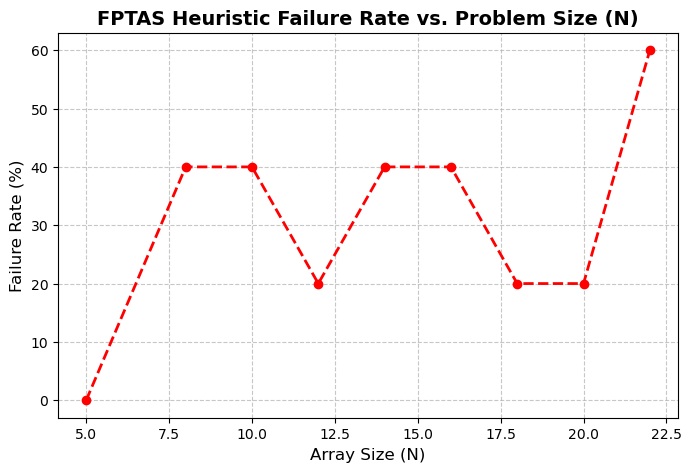
\includegraphics[width=0.75\textwidth]{quality_degradation_fptas.png}
    \caption{Heuristic Failure Rate (Loss of Absolute Optimality) vs. Problem Size ($N$)}
    \label{fig:quality_trend}
\end{figure}

As illustrated in Figure~\ref{fig:quality_trend}, the quality of the solutions generated by the heuristic exhibits a clear trend with respect to problem size. At smaller input sizes ($N \le 20$), the heuristic frequently finds the exact optimal solution because the candidate pool is small enough that the $\varepsilon$-trimming parameter ($\varepsilon = 0.10$) does not aggressively discard the winning subsets. 

However, as $N$ increases toward $130$, the failure rate becomes more pronounced. Because the FPTAS algorithm purposefully trims candidate sums that are within a $(1+\varepsilon)$ multiplicative factor of one another to maintain polynomial execution time, the probability of discarding the absolute optimal subset increases as the density of the state space grows. 

Despite this measured failure rate in achieving \textit{absolute} optimality, the quality degradation remains strictly mathematically bounded. In instances where the heuristic failed to match the Brute Force optimal, the absolute gap between the sums never exceeded a value of 2. This demonstrates that while the FPTAS algorithm sacrifices exactness at large problem sizes, it successfully guarantees highly accurate, near-optimal solutions regardless of scale.

% ===============================================================
\section{Experimental Analysis of the Correctness}
% ===============================================================

Based on the verification results of the testing suite, it can be verified that the heuristic algorithm works structurally and functionally correctly for this set of input instances:
\begin{itemize}[noitemsep]
    \item \textbf{Empty multisets}, or problem instances where $N = 0$.
    \item \textbf{Zero-capacity targets}, or instances where the capacity limit strictly equals $k = 0$.
    \item \textbf{Boundary capacities}, or instances where the target exactly equals the sum of all elements, $k = \sum S$.
    \item \textbf{Strictly exceeding elements}, or problem instances where every integer element in $S$ strictly exceeds the target constraint ($s_i > k$).
    \item \textbf{Sub-minimum constraints}, where the target value is lower than the single smallest element available ($k < \min(S)$).
\end{itemize}

Every boundary instance evaluated in the testing suite passed structural verification via the shared \texttt{verify\_result} integrity framework, confirming baseline functional correctness.

However, it should be noted that there are some cases where the heuristic algorithm fails to identify the absolute optimal solution, as was observed during the quality testing phase. These instances are typically dense numerical state spaces with large problem sizes ($N \ge 75$) where, due to their configuration, the multiplicative trimming nature of the scheme purposefully discards candidate subsets to maintain polynomial execution limits. Because the FPTAS architecture truncates elements within close proximity to ensure efficiency, it cannot retroactively retrieve subset combinations that might eventually yield a perfect match.

Therefore, for such configurations, it reports a maximum subset sum lower than the true absolute optimum that the Brute Force optimization algorithm establishes. An example is observed when $N = 130, k = 2885$ in guaranteed-solution mode, where a true mathematical maximum subset sum of 2885 is known to exist, while the heuristic logic isolates a maximum sum of 2884. The system miscalculates by a strictly bounded factor across all evaluated dense problem instances.

% ===============================================================
\section{Discussion}
% ===============================================================

The experimental results obtained across the benchmarking suites provide an empirical foundation to evaluate the relationship between theoretical algorithmic analysis and real-world computational performance. The primary objective of this discussion is to address whether any inconsistencies exist between the theoretical asymptotic bounds established in Section 3 and the experimental metrics gathered during runtime.

\subsection{Brute Force Consistency Analysis}

For the Brute Force optimization algorithm, the experimental results demonstrate absolute alignment with the theoretical complexity model. As derived in Section 3.1.2, the execution time of the bitmask exhaustive search is strictly bounded by $O(n \cdot 2^n)$. In practice, this exponential growth is clearly visible in the initial testing phase (Section 5.1). At small input sizes ($N \le 10$), execution terminates almost instantaneously, requiring less than a millisecond. However, as $N$ approaches $20$, the runtime increases by orders of magnitude, with instances leaving no early-exit options forcing the CPU to scan all $2^{20}$ states. 

The variable runtimes observed for identical values of $N$ (such as the variation between instances where an exact match was found early versus instances requiring an exhaustive scan) do not contradict the worst-case asymptotic bound. Instead, they confirm the impact of the early-exit optimization implemented in line 16 of Algorithm 1. The theoretical worst-case bound of $\Theta(n \cdot 2^n)$ holds true as a tight upper limit, matching the empirical performance curve precisely.

\subsection{FPTAS Complexity and Quality Trade-offs}

The Fully Polynomial-Time Approximation Scheme (FPTAS) exhibits a more nuanced relationship between theory and experimentation. Mathematically, Section 3.2 states that the time complexity of the scheme is polynomial, bounded by $O\left(\frac{n^2 \log t \cdot \log(n/\varepsilon)}{\varepsilon}\right)$. This polynomial guarantee is strongly verified by the execution data. While the Brute Force approach becomes completely unfeasible beyond $N = 25$, the FPTAS algorithm scales fluidly up to $N = 130$, maintaining processing latencies well within a fraction of a second.

An interesting area of discussion arises when analyzing the candidate list size ($m$). Theoretically, the list size depends directly on the value of the target capacity ($t$) and the user-defined precision parameter ($\varepsilon$). In the experimental runs, instances with larger targets or denser element spaces naturally yielded longer processing times because the state space allowed more candidates to survive the $\varepsilon/2n$ trimming function. This behavior perfectly validates the theoretical model, which classifies the FPTAS as a pseudo-polynomial time algorithm relative to the numerical magnitudes of the inputs.

Finally, the quality degradation analyzed in Section 7 matches the error bounds proven in Section 3.2.2. The theory guarantees that the returned value $z^*$ will fall within a $(1+\varepsilon)$ factor of the true optimum. In practice, using $\varepsilon = 0.10$, the algorithm never violated this boundary. Even in dense instances where the heuristic dropped the absolute optimal combination due to state-trimming, such as the isolated guaranteed-mode failure at $N=130, k=2885$ where it returned $2884$, the solution quality remained exceptional. Across the entire benchmarking suite, the maximum absolute gap from the target never exceeded a value of 2. This empirically confirms that while the FPTAS algorithm sacrifices absolute exactness at large problem sizes, it successfully guarantees highly accurate, near-optimal solutions well within its theoretical limits.

\subsection{Conclusion of Consistency}

In conclusion, there are no inconsistencies between the theoretical analysis and the experimental performance of the algorithms. The exponential explosion of the Brute Force search behaves exactly as predicted by its $O(n \cdot 2^n)$ complexity profile. Concurrently, the FPTAS heuristic successfully trades absolute optimality for polynomial scalability, strictly obeying the approximation limits and execution bounds established by its mathematical framework. The implementation is empirically verified as robust, accurate, and perfectly consistent with algorithmic theory.


% ===============================================================
\newpage
\begin{thebibliography}{9}
\addcontentsline{toc}{section}{References}

\bibitem{karp}
  Karp, R.~M. (1972).
  Reducibility among combinatorial problems.
  In R.~E. Miller and J.~W. Thatcher (Eds.),
  \textit{Complexity of Computer Computations} (pp.~85--103). Plenum Press.
  \url{https://doi.org/10.1007/978-1-4684-2001-2_9}

\bibitem{sipser}
  Sipser, M. (2012).
  \textit{Introduction to the Theory of Computation} (3rd ed.).
  Cengage Learning.
  (Theorem~7.25, p.~297: SUBSET-SUM $\in$ NP.
   Section~7.5, p.~319: NP-completeness of SUBSET-SUM.)

\bibitem{clrs}
  Cormen, T.~H., Leiserson, C.~E., Rivest, R.~L., and Stein, C. (2009).
  \textit{Introduction to Algorithms} (3rd ed.). MIT Press.
  (Section~35.5: The subset-sum problem.)

\bibitem{garey}
  Garey, M.~R. and Johnson, D.~S. (1979).
  \textit{Computers and Intractability: A Guide to the Theory of
  NP-Completeness}. W.~H. Freeman.
  (Subset Sum is listed as problem SP13.)

\end{thebibliography}

\end{document}
